%=============================================================================
%  CSE 465 Project Report, North South University
%  SKELETON. All structure, tables, figures and references are complete.
%  Every \writehere{} block is a paragraph for you to write.
%
%  Section order follows the required list:
%    Abstract, Introduction (ending in contribution bullets), Background Work
%    and Literature Review, Proposed Methodology, Experiments, Results,
%    Analysis, Conclusion, References, Code and data availability.
%
%  Compile in Overleaf with pdfLaTeX. Run it TWICE so the table of contents,
%  list of figures and cross references resolve.
%
%  Needs figures/fig3_main_result.png, figures/fig4_truncation.png,
%  figures/fig5_lengths.png
%=============================================================================
\documentclass[12pt,a4paper,oneside]{report}

\usepackage[T1]{fontenc}
\usepackage[utf8]{inputenc}
\usepackage{newtxtext,newtxmath}      % Times
\usepackage[margin=1in]{geometry}
\usepackage{setspace}
\usepackage{graphicx}
\usepackage{booktabs}
\usepackage{amsmath}
\let\Bbbk\relax                       % newtxmath already defines it
\usepackage{amssymb}
\usepackage{caption}
\usepackage{array}
\usepackage{enumitem}
\usepackage{tikz}
\usepackage{xcolor}
\usepackage[hidelinks]{hyperref}
\usepackage{titlesec}
\usepackage{tcolorbox}
\usetikzlibrary{shapes.geometric,arrows.meta,positioning,calc}

\onehalfspacing
\setlength{\parindent}{0pt}
\setlength{\parskip}{6pt}

\titleformat{\chapter}[hang]{\normalfont\Large\bfseries}{\thechapter}{1em}{}
\titlespacing*{\chapter}{0pt}{0pt}{20pt}

\captionsetup[figure]{font=small,labelfont=bf}
\captionsetup[table]{font=small,labelfont=bf}

\definecolor{nsublue}{RGB}{31,56,100}
\newcolumntype{L}[1]{>{\raggedright\arraybackslash}p{#1}}

%=============================================================================
% WRITING SLOT. Delete the whole \writehere{...} and put your paragraph there.
% \drafttrue shows the boxes while writing. \draftfalse hides them so you can
% check the real page count before submitting.
%=============================================================================
\newif\ifdraft
\drafttrue

\newcommand{\writehere}[2]{%
  \ifdraft
    \begin{tcolorbox}[colback=yellow!8,colframe=orange!55,
                      boxrule=0.6pt,left=6pt,right=6pt,top=4pt,bottom=4pt]
    {\small\textbf{WRITE: #1}\\[2pt]#2}
    \end{tcolorbox}
  \fi}

\begin{document}

%=============================================================================
% COVER
%=============================================================================
\begin{titlepage}
\centering
\vspace*{0.5cm}

{\large\bfseries Department of Electrical and Computer Engineering}\\[4pt]
{\large\bfseries North South University}\\[30pt]

{\large CSE 465 Course Project}\\[40pt]

{\LARGE\bfseries\color{nsublue}
Reasoning Termination, Not Reasoning Capability,\\[6pt]
Bounds Small Language Model Performance\\[6pt]
on Competition Mathematics\par}

\vspace{12pt}
{\large\itshape A budget forcing study of VibeThinker-3B on AIME 2025\par}

\vspace{50pt}
{\large\bfseries Abu Ahmad \quad ID\# 2121725042}\\[60pt]

{\large\bfseries Faculty Advisor:}\\[8pt]
{\large Dr. Nabeel Mohammed}\\[4pt]
{\large Professor}\\[4pt]
{\large ECE Department}\\[30pt]

{\large Summer, 2026}
\vfill
\end{titlepage}

%=============================================================================
\chapter*{APPROVAL}
\addcontentsline{toc}{chapter}{APPROVAL}

Abu Ahmad (ID \# 2121725042) from the Electrical and Computer Engineering
Department of North South University has worked on the CSE 465 project titled
``Reasoning Termination, Not Reasoning Capability, Bounds Small Language Model
Performance on Competition Mathematics'' under the supervision of
\textbf{Dr.\ Nabeel Mohammed} in partial fulfillment of the requirement for the
degree of Bachelor of Science in Engineering, and it has been accepted as
satisfactory.

\vspace{40pt}
\textbf{Supervisor's Signature}

\vspace{25pt}
\dotfill

Dr.\ Nabeel Mohammed\\
Professor\\
Department of Electrical and Computer Engineering\\
North South University\\
Dhaka, Bangladesh.

\vspace{35pt}
\textbf{Chairman's Signature}

\vspace{25pt}
\dotfill

Dr.\ Rajesh Palit\\
Professor and Chairman\\
Department of Electrical and Computer Engineering\\
North South University\\
Dhaka, Bangladesh.

%=============================================================================
\chapter*{DECLARATION}
\addcontentsline{toc}{chapter}{DECLARATION}

This is to declare that this project is my original work. No part of this work
has been submitted elsewhere partially or fully for the award of any other
degree or diploma. All project related information will remain confidential and
shall not be disclosed without the formal consent of the project supervisor.
Relevant previous works presented in this report have been properly
acknowledged and cited. The plagiarism policy, as stated by the supervisor, has
been maintained.

All numerical results reported in this report were measured by the author on the
hardware stated. No result is estimated or carried over from the source
publications. Where a quantity was not measured, it is labelled as such.

\vspace{50pt}
\textbf{Student's name and Signature}

\vspace{35pt}
1. Abu Ahmad

\vspace{10pt}
\rule{7cm}{0.4pt}

%=============================================================================
\chapter*{ACKNOWLEDGEMENTS}
\addcontentsline{toc}{chapter}{ACKNOWLEDGEMENTS}

\writehere{Acknowledgements, about 2 short paragraphs}{
Thank Dr.\ Nabeel Mohammed by name and say what he actually did. Then the ECE
department. Then, if you want, Weibo AI for releasing the model weights, the vLLM
project, and Kaggle for the free GPU, since without the free tier this project
could not have run. Close with family. Keep it short and specific.}

%=============================================================================
\chapter*{ABSTRACT}
\addcontentsline{toc}{chapter}{ABSTRACT}

\begin{center}
\textbf{Reasoning Termination, Not Reasoning Capability, Bounds Small Language
Model Performance on Competition Mathematics}
\end{center}

\writehere{Abstract, one paragraph, roughly 200 to 300 words}{
Your template forbids references, symbols, special characters, footnotes and
equations here, so write it in plain prose. Spell numbers out if you want to be
safe.
\\[4pt]
Cover these in order. (1) Topic: compact reasoning models now match much larger
ones on mathematics benchmarks. (2) Gap: those scores come from runs with no
token limit, and nobody reports what a realistic limit costs. (3) Method: you
evaluated a three billion parameter model on thirty competition problems, four
samples each, across budgets from one thousand to thirty two thousand tokens,
without touching the weights, logging why every generation stopped. (4) Results:
samples that finished were almost always correct, samples cut off scored zero for
lack of a written answer, and forcing the model to commit recovered seven to
thirteen points without ever destroying a correct answer. (5) Significance: any
benchmark that caps generation is measuring stopping behaviour and reporting it as
reasoning ability.}

%=============================================================================
\tableofcontents
\listoffigures
\listoftables
\clearpage

%=============================================================================
\chapter{Introduction}

\writehere{Opening, 3 to 4 paragraphs}{
Paragraph 1. What reasoning models are and why they improved. Reinforcement
learning with checkable rewards, cite \cite{deepseekr1} and \cite{deepseekmath}.
They produce very long chains of thought before answering.
\\[4pt]
Paragraph 2. VibeThinker-3B \cite{vibethinker}. Three billion parameters, built on
Qwen2.5-Coder-3B \cite{qwen25coder}, reports 91.4 on AIME 2025. Say why a model
this small mattering is interesting: it runs on one consumer card, which puts this
kind of reasoning within reach of a student rather than only a lab with a cluster.
Your own voice can show here.
\\[4pt]
Paragraph 3. The catch. Those scores come from runs with effectively no length
limit; the model card recommends a maximum of 40,960 tokens. Generating forty
thousand tokens per problem is slow on the hardware a student actually has. So the
accessibility argument contains an assumption nobody has checked.
\\[4pt]
Paragraph 4. The question. When the budget is cut and accuracy falls, what was
lost? Either the model needed those tokens to reach the answer (capability), or it
reached the answer early and kept verifying until the budget ran out
(termination). Say these are distinguishable by measurement, and that telling them
apart is the point of the project.}

\writehere{Purpose and constraints, 1 paragraph}{
State the purpose in one sentence: determine which failure mode explains the loss,
and test whether it can be recovered without retraining. Then the three
constraints that shaped everything: no weight modification, everything inside
Kaggle's free tier at thirty GPU hours a week, and every reported number measured
on that hardware rather than quoted from a paper.}

\writehere{Roadmap, 1 short paragraph}{
One sentence per chapter, from Chapter 2 through Chapter 7.}

The contributions of this project are the following.

\begin{itemize}

\item \writehere{Contribution 1, the diagnosis}{
Correct count equals finished count per problem. 95 of 120 samples finished and
essentially all were correct; of the 25 truncated, 23 scored zero for lack of a
parseable answer. State that the whole 91.4 to 80.8 shortfall is a truncation
artifact, and that to your knowledge this decomposition has not been reported for
a model in this size class.}

\item \writehere{Contribution 2, the intervention measured}{
Budget forcing \cite{s1} evaluated on a compact model at four budgets. Significant
at every budget by McNemar's test, and strictly non destructive: zero correct
answers destroyed across 139 interventions.}

\item \writehere{Contribution 3, a negative result}{
Three forcing phrasings are statistically indistinguishable, and the two stage
variant costs 2.1 times more compute for no gain. What matters is that the model
is made to commit, not how it is asked.}

\item \writehere{Contribution 4, upper bounds}{
A single forced sample beats the best of four unforced samples at the smaller
budgets, so forcing exceeds the ceiling of any method that only selects among
existing answers. Restricted to the recoverable population, forcing captures about
80 percent of what is there.}

\item \writehere{Contribution 5, the method that made it affordable}{
Prefix consistency. Generation is autoregressive, so the first N tokens of a long
run are what a budget N run would have produced. Generate once at the top budget,
save the traces, score every smaller budget on CPU at zero GPU cost. You validated
this rather than assuming it, and it cut the sweep by roughly a factor of three.}

\end{itemize}

%=============================================================================
\chapter{Background Work and Literature Review}

\section{Reinforcement learning for verifiable reasoning}

\writehere{2 paragraphs}{
First, DeepSeek-R1 \cite{deepseekr1} and the GRPO objective from DeepSeekMath
\cite{deepseekmath}. Rule based reinforcement learning over checkable rewards
produces long horizon reasoning with no step level supervision.
\\[4pt]
Second, VibeThinker-3B \cite{vibethinker} applying that in the small model regime.
Two facts matter to you: their evaluation imposes no output length cap, and their
reported weakness is knowledge heavy tasks rather than reasoning procedure. Then
say what is missing: neither the paper nor the model card reports how accuracy
degrades under a constrained budget, which is the regime anyone on modest hardware
occupies.}

\section{Inference time scaling}

\writehere{2 paragraphs}{
Self consistency \cite{selfconsistency} samples several chains and takes the
majority. Self refinement \cite{selfrefine} has the model critique and revise its
own output. VibeThinker's paper describes Claim Level Reliability Assessment.
\\[4pt]
Then the structural point, which carries your argument. All three select or refine
among candidate answers that already exist, so their achievable accuracy is
bounded by pass@k. Where samples agree, or produce no answer at all, they have
nothing to act on. Say you show in Chapter 5 that this bound is binding here.}

\section{Budget forcing}

\writehere{1 paragraph}{
Muennighoff et al. \cite{s1} introduced budget forcing in the s1 recipe: on
reaching a token budget, append a phrase that ends the reasoning segment and
demands an answer. Note what they did not do, because that is where your
contribution sits. They use it mainly to extend reasoning, combined with
supervised fine tuning, so its use as a standalone recovery mechanism on a frozen
model is not characterised, and nobody measures whether it can damage an output.}

\section{The gap}

The following observations follow from the literature above.

\begin{enumerate}[label=(\roman*)]
\item \writehere{Gap 1}{Published accuracies come from uncapped runs and the
degradation curve under realistic budgets is not characterised, even though
deployment cost is the main argument for compact models.}
\item \writehere{Gap 2}{Failure analyses report aggregate accuracy without
separating a wrong answer from an absent one, so two failure modes with different
remedies are scored identically at zero.}
\item \writehere{Gap 3}{Test time scaling methods are evaluated where samples
disagree, so their behaviour where samples agree or produce nothing is untested.}
\item \writehere{Gap 4}{Budget forcing has been evaluated as an extension
mechanism alongside fine tuning, not as a standalone recovery mechanism on a
frozen model, and no measurement exists of whether it can destroy a correct
output.}
\end{enumerate}

\writehere{Closing, 2 to 3 sentences}{
What those four gaps motivated: characterise the curve, decompose the failures,
evaluate forcing with an explicit test for harm, and bound the recovery against
both the selection ceiling and the extraction ceiling.}

%=============================================================================
\chapter{Proposed Methodology}

\section{Problem formulation}

Let $\pi$ be the frozen policy and $q$ a problem statement. Under an unconstrained
budget the model emits $y = (y_1,\dots,y_T)$ ending in an end of sequence token,
and an answer $a(y)$ is parsed from the final boxed expression. Under a budget $B$
the generation is cut at $\min(T,B)$ tokens.

Define the termination indicator
\begin{equation}
\tau_B(y) =
\begin{cases}
1, & T \le B \quad \text{(terminated on its own)}\\[2pt]
0, & T > B \quad \text{(truncated)}
\end{cases}
\label{eq:tau}
\end{equation}

and the correctness indicator
$c_B(y) = \mathbb{1}[\,a(y_{1:\min(T,B)}) = a^{\star}\,]$
where $a^{\star}$ is the ground truth.

\writehere{1 paragraph on what the two hypotheses predict}{
Under the capability hypothesis, truncated traces are wrong because the reasoning
is incomplete, so correctness should fall smoothly across both groups. Under the
termination hypothesis, correctness should be near total among terminated samples
and near zero among truncated ones. Point at Equation \eqref{eq:hypotheses} and
say this is what makes the two distinguishable by measurement.}

\begin{equation}
\Pr[\,c_B = 1 \mid \tau_B = 1\,] \approx 1,
\qquad
\Pr[\,c_B = 1 \mid \tau_B = 0\,] \approx 0
\label{eq:hypotheses}
\end{equation}

\section{Budget forcing}

\writehere{1 paragraph}{
Describe the procedure in words before the equation. Forcing acts only on
truncated samples: take the truncated prefix, append a fixed phrase that closes the
reasoning block and asks for the answer, decode greedily for a short continuation.
Samples that terminated on their own are left untouched, and say explicitly that
this is why the method cannot damage them. Note the cost, about five generated
tokens per intervened sample.}

\begin{equation}
\hat{a} = a\!\left(\pi\!\left(q \oplus y_{1:B} \oplus \phi\right)\right),
\qquad
\phi = \texttt{"</think> \ldots the final answer is \textbackslash boxed\{"}
\label{eq:forcing}
\end{equation}

\writehere{2 sentences on the three variants}{
Name them: a bare demand ($V_1$), a soft deadline ($V_3$), and a two stage variant
($V_2$) where the model first summarises what it established and only then is
asked for the answer. Say why you tested three rather than one.}

\section{Prefix consistency}

\writehere{1 paragraph}{
Explain Equation \eqref{eq:prefix} in plain words: the model generates left to
right and has no knowledge of its own budget, so the distribution of the first N
tokens does not depend on where generation was stopped. Then the consequence:
saving traces at the top budget lets every smaller budget be scored on CPU at zero
GPU cost. Say you validated this in Chapter 4 rather than assuming it.}

\begin{equation}
y_{1:N} \sim \pi(\cdot \mid q)\Big|_{\text{budget } N}
\;\;\overset{d}{=}\;\;
\left(y \sim \pi(\cdot \mid q)\Big|_{\text{budget } B}\right)_{1:N},
\qquad N \le B
\label{eq:prefix}
\end{equation}

\section{System design}

\writehere{1 short paragraph introducing Figure \ref{fig:pipeline}}{
Two or three sentences walking the reader through the diagram: generate once,
truncate on CPU to reach each budget, score, force only the truncated samples,
analyse.}

\begin{figure}[htbp]
\centering
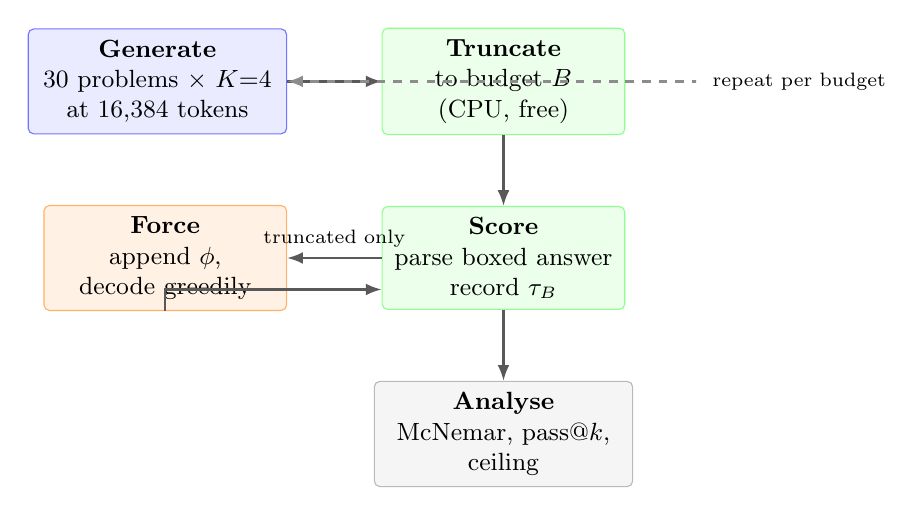
\begin{tikzpicture}[
  node distance=8mm,
  box/.style={draw,rounded corners=2pt,align=center,minimum height=11mm,
              inner sep=4pt,font=\small},
  gen/.style={box,fill=blue!8,draw=blue!55,text width=30mm},
  cpu/.style={box,fill=green!8,draw=green!45,text width=28mm},
  gpu/.style={box,fill=orange!10,draw=orange!60,text width=28mm},
  ana/.style={box,fill=gray!8,draw=gray!55,text width=30mm},
  ar/.style={-{Latex[length=2mm]},thick,draw=black!65}
]
\node[gen] (gen) {\textbf{Generate}\\30 problems $\times$ $K{=}4$\\at 16{,}384 tokens};
\node[cpu, right=12mm of gen] (trunc) {\textbf{Truncate}\\to budget $B$\\(CPU, free)};
\node[cpu, below=9mm of trunc] (score) {\textbf{Score}\\parse boxed answer\\record $\tau_B$};
\node[gpu, left=12mm of score] (force) {\textbf{Force}\\append $\phi$,\\decode greedily};
\node[ana, below=9mm of score] (stats) {\textbf{Analyse}\\McNemar, $\text{pass}@k$,\\ceiling};

\draw[ar] (gen) -- (trunc);
\draw[ar] (trunc) -- (score);
\draw[ar] (score) -- node[above,font=\scriptsize]{truncated only} (force);
\draw[ar] (force) |- ($(score.west)+(0,-4mm)$);
\draw[ar] (score) -- (stats);
\draw[ar,dashed,draw=black!45] (trunc.east) -- ++(9mm,0) |-
      node[right,font=\scriptsize,pos=0.25]{\;repeat per budget} (gen.east);
\end{tikzpicture}
\caption[Experimental pipeline]{Experimental pipeline. Generation runs once at the
largest budget. Smaller budgets come from truncating the stored traces on a CPU,
which costs nothing. Only the forcing step returns to the GPU, and it acts on
truncated samples alone.}
\label{fig:pipeline}
\end{figure}

\section{Statistical procedure}

\writehere{1 paragraph}{
The design is paired because the same samples are scored twice, before and after
the intervention, so an unpaired test would be the wrong tool. McNemar with
continuity correction \cite{mcnemar}, Equation \eqref{eq:mcnemar}, where $b$ is
samples that changed from incorrect to correct and $c$ the reverse. Say $c$ is of
independent interest because it measures whether the intervention can destroy a
correct answer. Wilson intervals \cite{wilson} for the ceiling proportions,
because the denominators are small and the normal approximation fails near unity.}

\begin{equation}
\chi^{2} = \frac{\left(|b - c| - 1\right)^{2}}{b + c},
\qquad \text{d.f.} = 1
\label{eq:mcnemar}
\end{equation}

%=============================================================================
\chapter{Experiments}

\section{Model, dataset and hardware}

\writehere{2 paragraphs}{
First: the model and the dataset. VibeThinker-3B, weights never modified. The 30
problem AIME 2025 set. Explain the substitution honestly, because a marker will
ask: AIME 2026 has no public dataset, so you used AIME 2025, and note this is an
advantage since the paper reports 91.4 for AIME 2025 and it let you validate your
harness. Integer answers between 0 and 999 mean exact matching with no judge model.
\\[4pt]
Second: the engine change. You started on HuggingFace transformers at 15.2 tokens
per second, which projected to over a hundred GPU hours and was not feasible. vLLM
\cite{vllm} raised it to 246.4 at $K{=}32$, a 16.2 times improvement, through
continuous batching and prefix sharing. Point at Table \ref{tab:tools}.}

\begin{table}[htbp]
\centering
\caption{Software and hardware components}
\label{tab:tools}
\small
\begin{tabular}{@{}L{2.3cm}L{3.5cm}L{3.0cm}L{5.6cm}@{}}
\toprule
\textbf{Tool} & \textbf{Function} & \textbf{Alternatives} & \textbf{Why selected} \\
\midrule
vLLM & Inference engine & HF \texttt{transformers}, TensorRT-LLM &
$16.2\times$ faster through continuous batching and prefix sharing; the workload
is many samples from one prompt, its best case \\
\addlinespace
Tesla T4 (16\,GB) & Accelerator & A100, TPU v4 & The only hardware on the free
tier; forces \texttt{float16} and rules out FlashAttention-2 \\
\addlinespace
VibeThinker-3B & Subject model & Qwen3-4B, Phi-4-mini & Frontier accuracy at 3B;
a published AIME 2025 score allows harness validation \\
\addlinespace
\texttt{math-ai/} \texttt{aime25} & Benchmark & AIME 2024, HMMT & Integer answers
allow exact matching against a published reference number \\
\addlinespace
Kaggle Notebooks & Compute platform & Colab, Lambda Labs & 30 GPU hours per week
at no cost; batch execution survives disconnection \\
\bottomrule
\end{tabular}
\end{table}

\writehere{1 paragraph on the T4 constraints}{
Three consequences of the card being Turing, compute capability 7.5.
FlashAttention-2 needs 8.0 or above so vLLM falls back to a Triton backend.
bfloat16 is unsupported so float16 is mandatory. And the KV cache holds 192,272
tokens at 90 percent utilisation, so concurrency is that divided by the context
window, Equation \eqref{eq:concurrency}, which is why a 32k context sustained 60 to
71 tokens per second while an 8k context sustained 246.}

\begin{equation}
\text{concurrency} = \frac{192{,}272}{\texttt{max\_model\_len}}
\label{eq:concurrency}
\end{equation}

\section{Protocol}

\writehere{2 paragraphs}{
One: the controls. Decoding parameters frozen across every arm, temperature 1.0,
top\_p 0.95, seed 0, $K$ equals 4 giving 120 samples per condition. Prompt from the
model's own chat template. Answer extraction finds the final boxed expression with
a brace depth parser. One shared implementation across all arms so a change cannot
apply to only one condition. Budgets of 4,096, 8,192, 16,384 and 32,768 tokens.
\\[4pt]
Two: termination logging, and why it is the important part. Distinguishing a wrong
answer from an absent one is what makes Equation \eqref{eq:hypotheses} testable.
Aggregate accuracy alone cannot support the central claim, which is why the harness
records the stop reason for every sample.}

\section{Compute expenditure}

\begin{table}[htbp]
\centering
\caption{Measured compute expenditure}
\label{tab:compute}
\small
\begin{tabular}{@{}lrl@{}}
\toprule
\textbf{Stage} & \textbf{GPU hours} & \textbf{Purpose} \\
\midrule
Setup and probes & 1.50 & Environment audit, throughput, diagnosis \\
Baseline (32K) & 8.87 & 30 problems $\times$ $K{=}4$, unconstrained budget \\
Budget forcing (4K, 8K) & 2.06 & First forcing measurement \\
Forcing variants (16K) & 8.89 & Trace generation and six forcing passes \\
Trace analysis & 0.00 & CPU only; fine grained curve and figures \\
Paired analysis & 1.28 & McNemar contingency at 8K and 16K \\
Upper bounds & 0.00 & CPU only; $\text{pass}@k$ and extraction ceiling \\
\midrule
\textbf{Total} & \textbf{22.60} & \\
\bottomrule
\end{tabular}
\end{table}

\section{Harness validation}

\writehere{2 paragraphs}{
First check: your baseline reproduction gave 80.8 against the published 91.4. Make
the point that the direction matters. Your figure is lower, which argues against
contamination inflating anything.
\\[4pt]
Second check: the prefix consistency identity of Equation \eqref{eq:prefix} tested
directly. An 8,192 token condition measured two ways, a genuine 8k run and
truncated 16k traces, gave 54.2 and 55.8 percent. Two samples out of 120, within
noise at temperature 1.0. Say every later budget result depends on this identity
holding.}

%=============================================================================
\chapter{Results}

\section{Termination against correctness}

\writehere{1 paragraph introducing Table \ref{tab:decomp}}{
Say what the reader should look at: the two columns coincide.}

\begin{table}[htbp]
\centering
\caption{Correct samples against naturally terminated samples, 32K budget}
\label{tab:decomp}
\small
\begin{tabular}{@{}crrl@{}}
\toprule
\textbf{Problem} & \textbf{Correct} & \textbf{Terminated} & \textbf{Note} \\
\midrule
8  & 2/4 & 2/4 & \\
13 & 0/4 & 0/4 & all truncated \\
14 & 0/4 & 0/4 & all truncated \\
19 & 2/4 & 2/4 & \\
26 & 3/4 & 3/4 & \\
27 & 1/4 & 1/4 & \\
29 & 0/4 & 0/4 & all truncated \\
\midrule
21 problems & 4/4 & 4/4 & solved by every sample \\
\bottomrule
\end{tabular}
\end{table}

\writehere{1 paragraph, arithmetic only, save interpretation for Chapter 6}{
All 21 fully solved problems also terminated on all four samples, contributing 84
samples. Aggregating, 97 correct and 95 terminated, so among the 95 that
terminated essentially every one was correct. Of the 25 truncated, 23 scored zero.
Keep this factual here.}

\section{Accuracy against budget}

\begin{figure}[htbp]
\centering
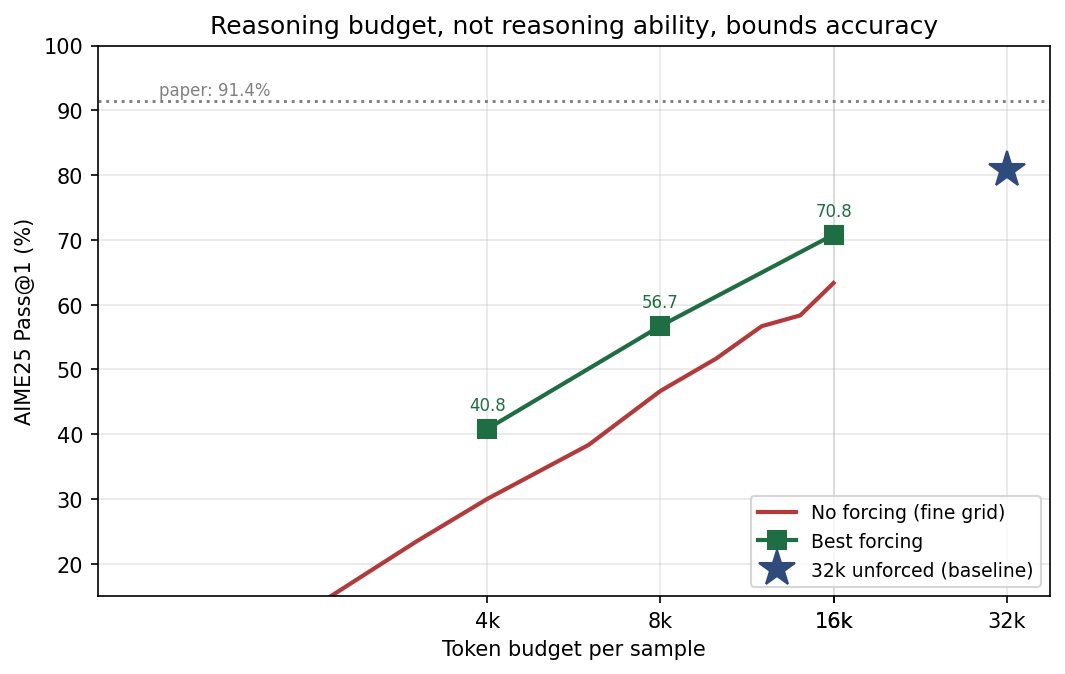
\includegraphics[width=0.85\textwidth]{figures/fig3_main_result.png}
\caption[Accuracy against generation budget]{Accuracy against generation budget,
with and without budget forcing. The dotted line marks the accuracy reported in
\cite{vibethinker} under an unconstrained budget.}
\label{fig:main}
\end{figure}

\begin{table}[htbp]
\centering
\caption{Accuracy and truncation rate against budget, no forcing}
\label{tab:curve}
\small
\begin{tabular}{@{}rrr@{\hspace{2.2em}}rrr@{}}
\toprule
\textbf{Budget} & \textbf{Pass@1} & \textbf{Truncated} &
\textbf{Budget} & \textbf{Pass@1} & \textbf{Truncated} \\
\midrule
1K & 3.3\%  & 100.0\% & 8K  & 46.7\% & 67.5\% \\
2K & 13.3\% & 98.3\%  & 10K & 51.7\% & 63.3\% \\
3K & 23.3\% & 92.5\%  & 12K & 56.7\% & 59.2\% \\
4K & 30.0\% & 87.5\%  & 14K & 58.3\% & 53.3\% \\
6K & 38.3\% & 77.5\%  & 16K & 63.3\% & 48.3\% \\
\bottomrule
\end{tabular}
\end{table}

\begin{figure}[htbp]
\centering
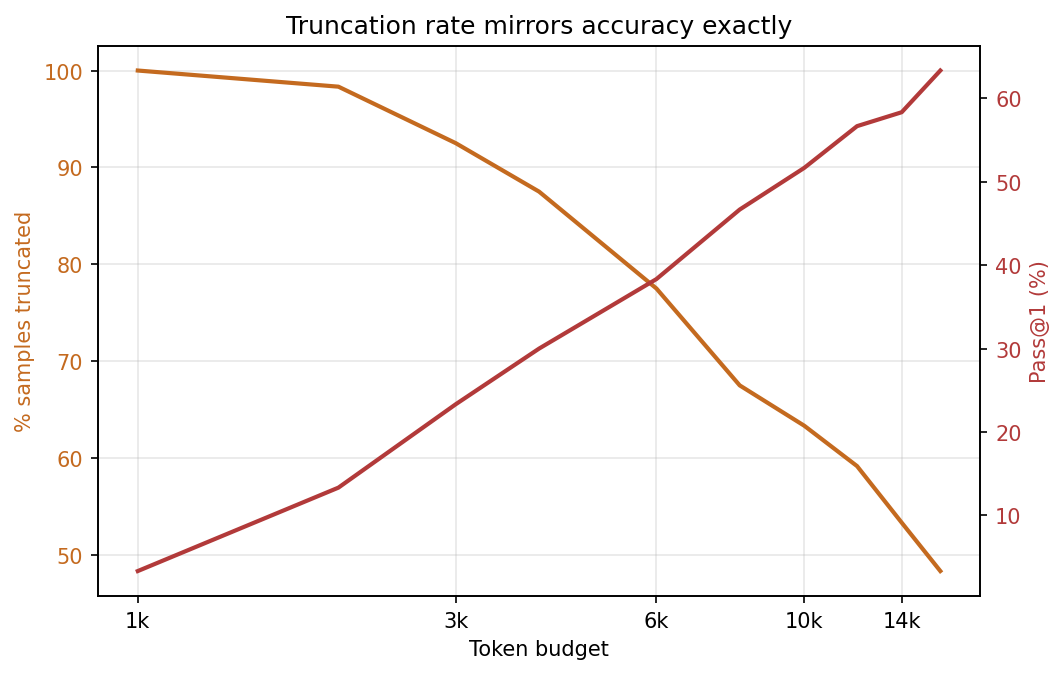
\includegraphics[width=0.85\textwidth]{figures/fig4_truncation.png}
\caption[Truncation rate against accuracy]{Truncation rate and accuracy move
inversely with budget. The left axis gives the percentage of samples cut off by the
budget; the right axis gives Pass@1 over the same samples.}
\label{fig:trunc}
\end{figure}

\writehere{1 paragraph}{
State the curve factually and note one thing a reader will otherwise miss:
accuracy exceeds the natural termination rate by 12 to 18 points at every budget,
because the model sometimes writes an intermediate boxed expression mid derivation
which the parser recovers even though the trace never terminated. The unforced
baseline therefore already captures some truncated but answered samples.}

\begin{figure}[htbp]
\centering
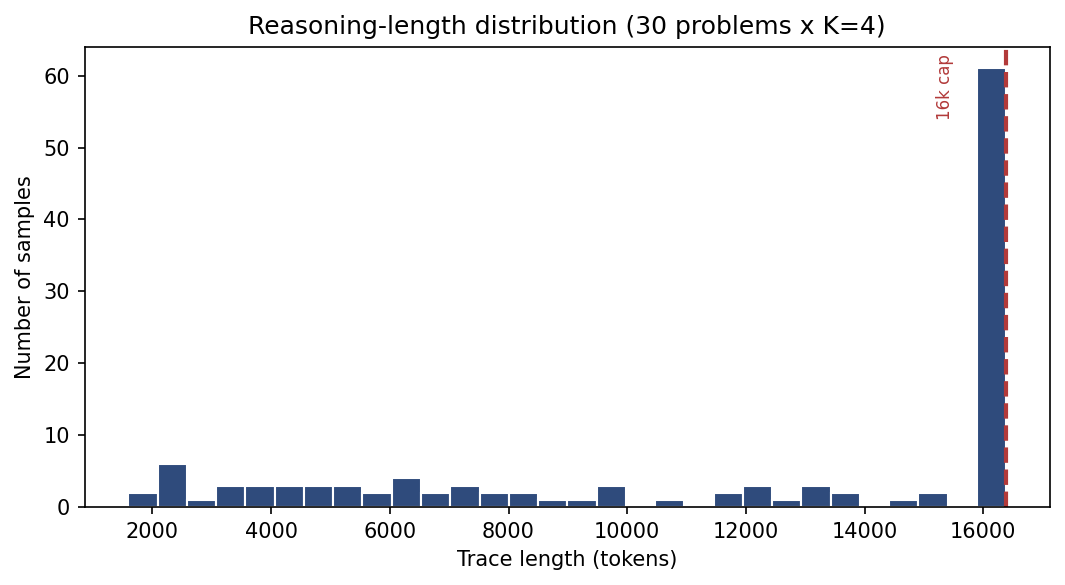
\includegraphics[width=0.85\textwidth]{figures/fig5_lengths.png}
\caption[Reasoning length distribution]{Distribution of reasoning trace lengths
over 30 problems $\times$ $K{=}4$ samples. The distribution is right censored at
16{,}384 tokens; the mass at the cap is an artifact of the imposed limit, not the
model stopping on its own.}
\label{fig:lengths}
\end{figure}

\section{Effect of budget forcing}

\begin{table}[htbp]
\centering
\caption{Effect of budget forcing on AIME 2025 Pass@1}
\label{tab:main}
\small
\begin{tabular}{@{}lrrrc@{}}
\toprule
\textbf{Budget} & \textbf{No forcing} & \textbf{With forcing} & \textbf{Gain} &
\textbf{McNemar $p$} \\
\midrule
4K  & 27.5\% / 30.0\% & 40.8\% & $+13.3$ & not run \\
8K  & 46.7\%          & 55.8\% & $+9.1$  & $\mathbf{0.0026}$ \\
16K & 63.3\%          & 70.8\% & $+7.5$  & $\mathbf{0.0077}$ \\
32K & 80.8\%          & not measured & & \\
\bottomrule
\end{tabular}
\end{table}

\writehere{1 paragraph}{
The gain is significant at every budget where the paired test could be applied.
Explain the two baselines in the 4K row honestly: that budget was measured twice,
once by a dedicated run at 27.5 percent and once by truncating traces at 30.0
percent. Three samples apart, within noise, but different experiments, so they
should not be plotted as one series.}

\section{Test for harm}

\begin{table}[htbp]
\centering
\caption{Paired contingency for budget forcing, truncated samples only}
\label{tab:paired}
\small
\begin{tabular}{@{}lrrrrrr@{}}
\toprule
\textbf{Budget} & \textbf{Truncated} & \textbf{$b$ rescued} &
\textbf{$c$ damaged} & \textbf{right$\to$right} & \textbf{$\chi^2$} & \textbf{$p$} \\
\midrule
8K  & 81 & 11 & \textbf{0} & 17 & 9.09 & 0.0026 \\
16K & 58 & 9  & \textbf{0} & 14 & 7.11 & 0.0077 \\
\bottomrule
\end{tabular}
\end{table}

\writehere{1 paragraph, factual}{
Across 139 interventions $c$ equals zero. Note that 31 truncated traces already
contained a correct boxed expression and forcing re derived the identical value for
every one. Save the explanation for Chapter 6.}

\section{Sensitivity to the forcing phrase}

\begin{table}[htbp]
\centering
\caption{Comparison of forcing phrasings}
\label{tab:variants}
\small
\begin{tabular}{@{}lrrr@{\hspace{2em}}rr@{}}
\toprule
& \multicolumn{3}{c}{\textbf{Pass@1}} & \multicolumn{2}{c}{\textbf{Cost (min)}} \\
\cmidrule(lr){2-4}\cmidrule(l){5-6}
\textbf{Budget} & $V_1$ bare & $V_3$ deadline & $V_2$ summarise &
$V_1$ & $V_2$ \\
\midrule
8K  & 55.8\% & 55.8\% & 56.7\% & 21.2 & 47.8 \\
16K & 70.8\% & 70.8\% & 70.8\% & 54.9 & 117.3 \\
\bottomrule
\end{tabular}
\end{table}

\writehere{1 paragraph, factual}{
Identical at 16K. The 0.9 point lead at 8K is one sample out of 120. $V_2$ costs
2.1 times more compute at both budgets.}

\section{Upper bounds}

\begin{table}[htbp]
\centering
\caption{Budget forcing against the selection oracle}
\label{tab:oracle}
\small
\begin{tabular}{@{}lrr@{}}
\toprule
\textbf{Budget} & \textbf{Unforced pass@4 (oracle)} & \textbf{Forced pass@1} \\
\midrule
4K  & 40.0\% & \textbf{40.8\%} \\
8K  & 53.3\% & \textbf{55.8\%} \\
16K & \textbf{73.3\%} & 70.8\% \\
\bottomrule
\end{tabular}
\end{table}

\begin{table}[htbp]
\centering
\caption{Extraction ceiling on the recoverable population}
\label{tab:ceiling}
\small
\begin{tabular}{@{}lrrrrrrrc@{}}
\toprule
\textbf{Budget} & \textbf{Trunc.} & \textbf{Already ok} & \textbf{Rescuable} &
\textbf{Has ans.} & \textbf{FP} & \textbf{Ceiling} & \textbf{Rescued} &
\textbf{Captured} \\
\midrule
8K  & 81 & 17 & 64 & 16 & 2 & 14 & 11 & 78.6\% \\
16K & 58 & 14 & 44 & 11 & 0 & 11 &  9 & 81.8\% \\
\bottomrule
\end{tabular}
\end{table}

\writehere{2 paragraphs, factual}{
One: at 4K and 8K a single forced sample beats the best of four unforced ones; at
16K the ordering reverses. State the caveat: this compares forced pass@1 against
unforced pass@4, and forced pass@4 was not computed.
\\[4pt]
Two: forcing captures 78.6 percent at 8K and 81.8 at 16K of the recoverable
population, with Wilson intervals of roughly 52 to 92 and 52 to 95 on populations
of 14 and 11. The false positive control ran 0 to 4.9 percent against a signal of
32 to 41 percent. Only 16 of 64 rescuable traces at 8K and 11 of 44 at 16K mention
the correct answer anywhere in their final fifth.}

%=============================================================================
\chapter{Analysis}

\section{Termination, not capability}

\writehere{2 paragraphs}{
First: interpret Table \ref{tab:decomp}. The pattern is what Equation
\eqref{eq:hypotheses} predicts under the termination hypothesis and is inconsistent
with the capability hypothesis, which predicts smooth degradation across both
groups. So the 91.4 to 80.8 shortfall is a truncation artifact rather than a
reasoning deficit.
\\[4pt]
Second: the worked example, which is the most convincing thing in the report.
Problem 1, answer 588. The model derives $AB = 28$ and $AC = 91$, sets up
coordinates, concludes the heptagon area equals the triangle area, and the value 588
appears in its working. Then it keeps verifying and never writes a boxed answer
before the budget expires. The reasoning succeeded. Only the act of stating the
result failed.}

\section{Why forcing cannot do harm}

\writehere{2 paragraphs}{
First: explain the zero using the right to right column. Thirty one truncated
traces already contained a correct boxed expression, and forcing overwrote every one
and re derived the identical value. Once the model has established a result firmly
enough to state it once, being made to state it again reproduces it, because the
working is still in its context.
\\[4pt]
Second: the consequence. A hybrid policy that preserves an existing answer and
forces only when none is present scores identically, so the extra logic is
unnecessary. Say you built it and discarded it, because that is what happened.}

\section{Why the phrasing does not matter}

\writehere{2 paragraphs}{
First: interpret Table \ref{tab:variants}. What the intervention supplies is
permission to stop, not a better prompt, so elaborating the request adds cost
without adding information. The information the model needs is already in its own
trace.
\\[4pt]
Second: the cost caveat, and be careful here. Forcing's wall clock cost is
dominated by prefill, that is re reading the stored trace, because the forcing step
itself generates about five tokens. An implementation that kept the KV cache would
make forcing nearly free, so these timings are not an intrinsic cost of the method.}

\section{What forcing can and cannot recover}

\writehere{3 paragraphs}{
One: the two worked examples together. Problem 1, answer 588, where three of four
summaries contain genuine derived quantities and forcing yields 588. Problem 13,
answer 60, where the summaries are still setting up the problem and forcing yields
confident but wrong values of 124 and 184.
\\[4pt]
Two: the generalisation. Budget forcing recovers answers already latent in the
trace and cannot manufacture reasoning that has not occurred. Show that this single
statement accounts for all four findings: the gain is real because latent answers
are common, the gain is bounded because most failures are genuinely incomplete,
forcing is non destructive because a latent answer is stable under re elicitation,
and the phrasing is irrelevant because what is supplied is permission to conclude.
\\[4pt]
Three: where the headroom actually is. Only about a quarter of rescuable traces
mention the answer at all, so roughly three quarters of failures never derived it
and no extraction procedure could recover them. The remaining opportunity is in
generating reasoning, not reading it out.}

\section{Implications for evaluation practice}

\writehere{1 paragraph, and say what you actually think}{
Any benchmark that caps generation on a long horizon reasoning model measures a
composite of reasoning ability and stopping behaviour and reports it as reasoning
ability alone. Under such protocols this trivially cheap intervention is worth 7 to
13 points, which is larger than the margin separating many published systems. This
is the place in the report where a judgement of your own belongs.}

%=============================================================================
\chapter{Conclusion}

\writehere{2 paragraphs}{
One: restate the question and the answer. You asked whether the accuracy loss under
a constrained budget reflects a failure of reasoning or of termination, and the two
separate cleanly: samples that terminated were almost always correct, truncated
samples scored zero for lack of a written answer.
\\[4pt]
Two: what forcing achieved. 7.5 to 13.3 points, significant at every budget by
McNemar, never converted a correct answer into an incorrect one across 139
interventions, three phrasings indistinguishable, a single forced sample beating the
best of four unforced ones at the smaller budgets, and roughly 80 percent of
recoverable answers captured. End on the compute figure: the whole study took 22.6
GPU hours on freely available hardware.}

\section{Limitations}

\begin{itemize}
\item \writehere{Sample and seed}{One model, one benchmark, one seed. Intervals are
binomial over 120 samples with no run to run variance estimate, so the defensible
claim is that the effect exceeds plausible sampling noise, not that it replicates.}
\item \writehere{K equals 4}{Adequate for pass@1 but limits per problem resolution
and widens every interval.}
\item \writehere{Ceiling population}{The extraction ceiling rests on 11 to 14
samples, so its 95 percent interval spans roughly 52 to 95 percent.}
\item \writehere{Benchmark substitution}{AIME 2026 was unavailable publicly so AIME
2025 was used. It predates the subject publication and was within its evaluation
scope. Your accuracy came in below theirs, which argues against contamination, but
no independent decontamination check was performed.}
\item \writehere{Context length not held constant}{max\_model\_len differed across
arms, 10240, 18432 and 32768, for memory reasons. It does not affect sampling logits
and an 8K condition measured under two values agreed within noise, but it was not
controlled and you should not claim it was.}
\item \writehere{Cost figures are implementation bound}{Forcing's wall clock cost is
prefill from reprocessing each stored trace. A cache reusing implementation would
make it nearly free.}
\item \writehere{Two conditions not measured}{Forcing at 32K was not run; the trend
extrapolates to roughly plus 5 but that is extrapolation. Forced pass@4 was not
computed, so the oracle comparison is not like for like.}
\item \writehere{A superseded metric}{An earlier ceiling estimate divided rescued
samples by a denominator that proved to coincide with the already correct set,
making numerator and denominator disjoint. It was retracted and replaced by Table
\ref{tab:ceiling}. Keep this in.}
\end{itemize}

\section{Future work}

\writehere{4 short paragraphs, one per direction}{
Cache reusing forcing: keeping the KV cache instead of reprocessing the prefix would
cut the cost to roughly the five tokens it actually generates.
\\[4pt]
Learned termination: since about three quarters of failures never derive the answer,
the larger opportunity is making the model conclude sooner rather than extracting
more from incomplete traces.
\\[4pt]
Generality: one model, one benchmark. Whether the decomposition holds for other
compact reasoning models, and on code generation as well as mathematics, is open.
The prefix consistency identity makes such a sweep affordable.
\\[4pt]
Evaluation protocol: publishing the truncation rate alongside accuracy would cost
nothing and make results across different budgets comparable.}

%=============================================================================
\begin{thebibliography}{99}
\addcontentsline{toc}{chapter}{References}

\bibitem{vibethinker}
S. Xu, S. Liu, W. Wang, J. Min, Y. Dai, Z. Yin, Y. Chen, X. Zhou and J. Zhang,
``VibeThinker-3B: Exploring the frontier of verifiable reasoning in small language
models,'' \emph{arXiv preprint} arXiv:2606.16140, 2026.

\bibitem{s1}
N. Muennighoff, Z. Yang, W. Shi, X. L. Li, L. Fei-Fei, H. Hajishirzi,
L. Zettlemoyer, P. Liang, E. Cand\`{e}s and T. Hashimoto, ``s1: Simple test time
scaling,'' \emph{arXiv preprint} arXiv:2501.19393, 2025.

\bibitem{deepseekr1}
D. Guo, D. Yang, H. Zhang, J. Song, R. Zhang, R. Xu, Q. Zhu, S. Ma, P. Wang and
X. Bi, ``DeepSeek-R1: Incentivizing reasoning capability in LLMs via reinforcement
learning,'' \emph{arXiv preprint} arXiv:2501.12948, 2025.

\bibitem{deepseekmath}
Z. Shao, P. Wang, Q. Zhu, R. Xu, J. Song, X. Bi, H. Zhang, M. Zhang, Y. K. Li and
Y. Wu, ``DeepSeekMath: Pushing the limits of mathematical reasoning in open language
models,'' \emph{arXiv preprint} arXiv:2402.03300, 2024.

\bibitem{selfconsistency}
X. Wang, J. Wei, D. Schuurmans, Q. Le, E. Chi, S. Narang, A. Chowdhery and D. Zhou,
``Self consistency improves chain of thought reasoning in language models,''
\emph{International Conference on Learning Representations}, 2023.

\bibitem{selfrefine}
A. Madaan, N. Tandon, P. Gupta, S. Hallinan, L. Gao, S. Wiegreffe, U. Alon,
N. Dziri, S. Prabhumoye and Y. Yang, ``Self-Refine: Iterative refinement with self
feedback,'' \emph{Advances in Neural Information Processing Systems}, vol. 36,
pp. 46534 to 46594, 2023.

\bibitem{qwen25coder}
B. Hui, J. Yang, Z. Cui, J. Yang, D. Liu, L. Zhang, T. Liu, J. Zhang, B. Yu and
K. Dang, ``Qwen2.5-Coder technical report,'' \emph{arXiv preprint} arXiv:2409.12186,
2024.

\bibitem{vllm}
W. Kwon, Z. Li, S. Zhuang, Y. Sheng, L. Zheng, C. H. Yu, J. Gonzalez, H. Zhang and
I. Stoica, ``Efficient memory management for large language model serving with
PagedAttention,'' \emph{Proceedings of the 29th Symposium on Operating Systems
Principles}, pp. 611 to 626, 2023.

\bibitem{mcnemar}
Q. McNemar, ``Note on the sampling error of the difference between correlated
proportions or percentages,'' \emph{Psychometrika}, vol. 12, no. 2, pp. 153 to 157,
1947.

\bibitem{wilson}
E. B. Wilson, ``Probable inference, the law of succession, and statistical
inference,'' \emph{Journal of the American Statistical Association}, vol. 22,
no. 158, pp. 209 to 212, 1927.

\end{thebibliography}

%=============================================================================
\chapter*{Code and Data Availability}
\addcontentsline{toc}{chapter}{Code and Data Availability}

The analysis code, the measured result files and all 120 reasoning traces are held
in the project repository:

\begin{center}
\url{https://github.com/abuahmad369/llm-budget-forcing}
\end{center}

A public write up, the result files and an interactive explorer holding all 120
traces are available at:

\begin{center}
\url{https://github.com/abuahmad369/reasoning-termination}\\[4pt]
\url{https://abuahmad369.github.io/reasoning-termination/}
\end{center}

\end{document}
